\section{ Fundamento teórico}
\subsection{ Esfuerzo, deformación y módulos de elasticidad}
En muchos casos, los procesos de estiramiento, compresión, flexión, torcedura y corte de los cuerpos reales son muy importante, por lo que no pueden ser despreciables.\\
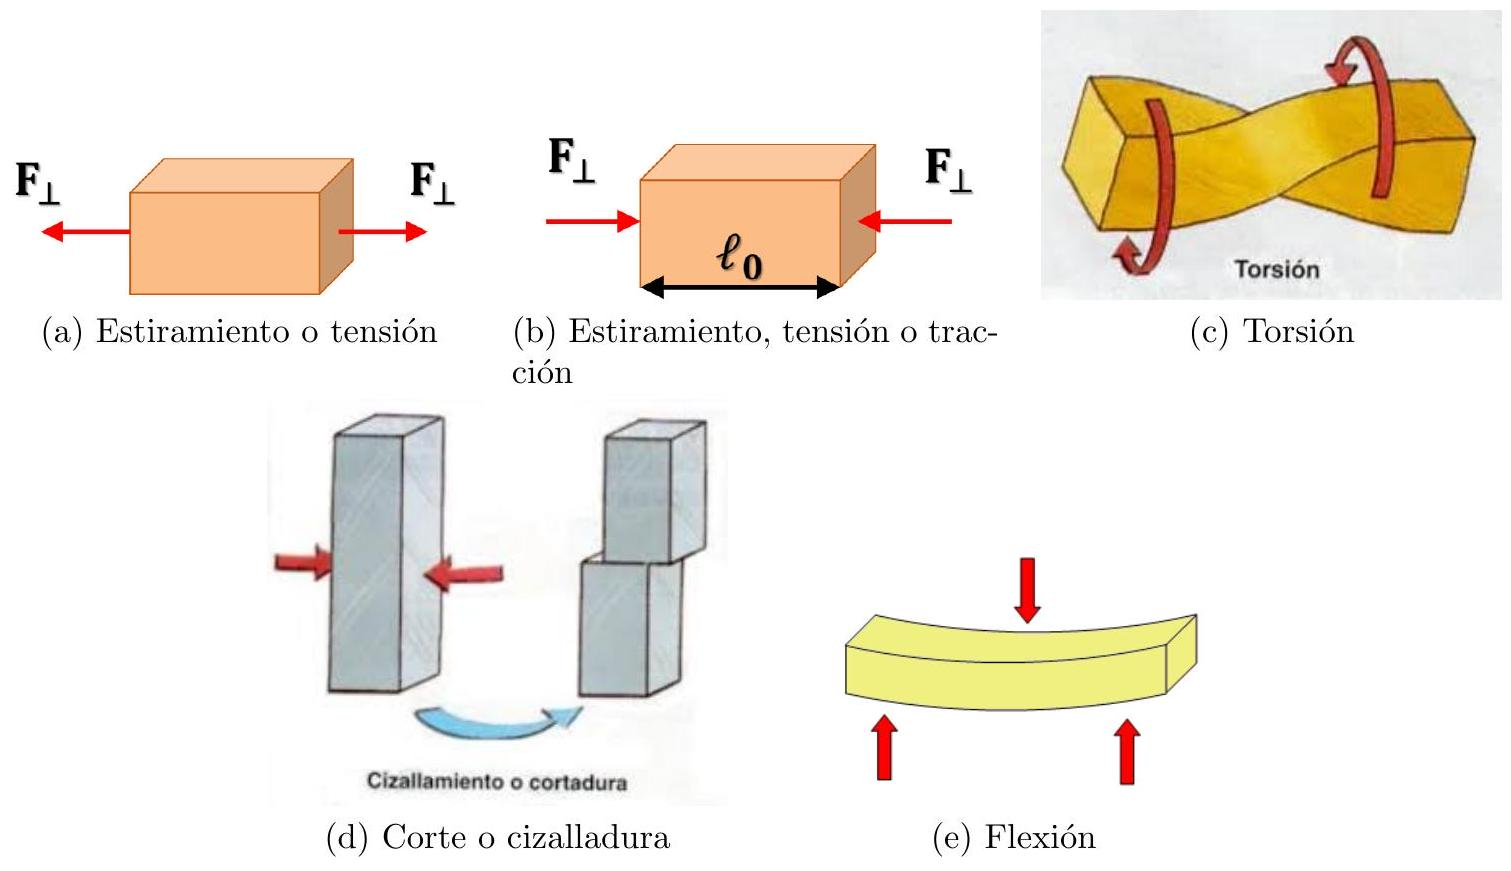
\includegraphics[max width=\textwidth, center]{2025_04_28_a9941da8947ada55c6c9g-02}

Todo cuerpo sólido se deforma bajo la acción de fuerzas, y al cesar estas, tiende a recuperar su forma, esta tendencia se denomina elasticidad. En la realidad, no hay cuerpo perfectamente elástico o inelástico, solo cuerpo con deformaciones con parte elástica y permanente. Generalmente, si las fuerzas no sobrepasan determinados valores, los cuerpos pueden considerarse elásticos.

\subsection{ Módulo de elasticidad}
Para cada clase de deformación, se introducen las cantidades esfuerzo( $\sigma$ )(intensidad de fuerzas que causan la deformación) y deformación unitaria( $(\varepsilon)$ (cambio de forma resultante). Si tenemos esfuerzo y deformación unitaria pequeños, podemos establecer que son directamente proporcionales(comprobado experimentalmente). Luego, dentro de este intervalo, definimos al módulo de elasticidad $(M)$ como :


\begin{equation*}
M=\frac{\sigma}{\varepsilon} \tag{1}
\end{equation*}


A este comportamiento se le denomina"Ley de Hooke".

\subsection{ Esfuerzo y deformación de tensión y compresión}
\subsection{ Esfuerzo y deformación por tensión}
Cuando un cuerpo se somete a fuerzas que tiran de sus extremos, tiende a incrementar su longitud respecto a la dirección de estas fuerzas; en el caso de una barra tenemos:\\
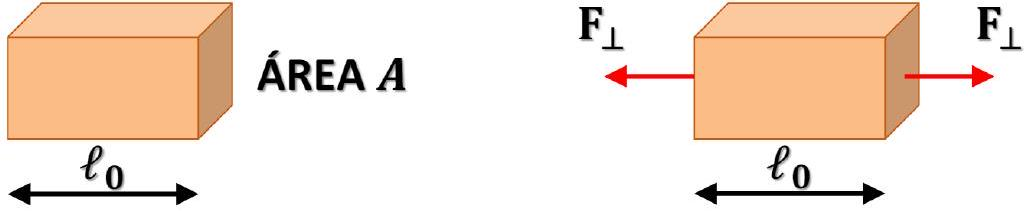
\includegraphics[max width=\textwidth, center]{2025_04_28_a9941da8947ada55c6c9g-03(1)}

Figura 1: Estiramiento de barra\\
Definimos al esfuerzo de tensión $(\sigma)$ como cociente entre fuerza $\left(F_{\perp}\right)$ y área transversal $(A)$ :


\begin{equation*}
\sigma=\frac{F_{\perp}}{A} \tag{2}
\end{equation*}


Cantidad escalar, puesto que solo abajamos con la intensidad de la fuerza $\left(\frac{N}{m^{2}}\right)(P a)$.\\
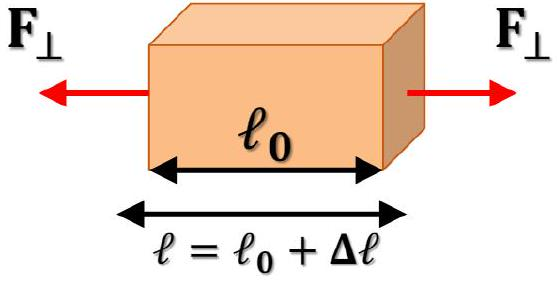
\includegraphics[max width=\textwidth, center]{2025_04_28_a9941da8947ada55c6c9g-03}

Figura 2: Longitud final de barra\\
Sea $\ell_{0}$ la longitud inicial y $\ell$ la longitud final, tenemos que la variación de longitud $\Delta \ell=\ell-\ell_{0}$ de la barra es positiva, al incrementarse por tensión. Luego tenemos que la deformación unitaria( $(\varepsilon)$ es:


\begin{equation*}
\varepsilon=\frac{\Delta \ell}{\ell_{0}} \tag{3}
\end{equation*}


Notamos que $\varepsilon$ es adimensional.\\
Si tenemos que esfuerzo y deformación unitaria son pequeños, entonces definimos el módulo de Young $(Y)$ como el módulo de elasticidad de tensión:

$$
\begin{aligned}
Y & =\frac{\sigma}{\varepsilon} \\
& =\frac{F_{\perp} \ell_{0}}{\Delta \ell A}
\end{aligned}
$$

Notamos que el módulo de young y esfuerzo tienen las mismas unidades. Si $Y$ es muy grande, el cuerpo no se estira mucho, para el caso contrario, hay más estiramiento.

\subsection{ Esfuerzo y deformación por compresión}
Similar al esfuerzo y deformación por tensión, se definen las cantidades esfuerzo de compresión $(\sigma)$ y deformación unitaria por compresión $(\varepsilon)$. La deformación por compresión se produce cuando las fuerzas empujan a la barra, en lugar de jalar.\\
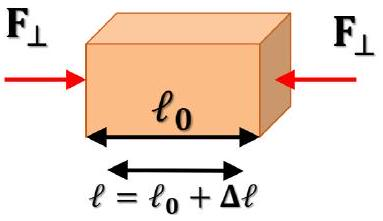
\includegraphics[max width=\textwidth, center]{2025_04_28_a9941da8947ada55c6c9g-04(1)}

Figura 3: Compresión de barra\\
Como $\ell<\ell_{0}$ entonces $\Delta \ell<0$, luego la deformación unitaria cambia de signo para evitar discrepancias entre el valor del módulo de elasticidad, por lo que $\varepsilon=-\frac{\Delta \ell}{\ell_{0}}$. La ley de Hooke se cumple para esfuerzos pequeños, luego el módulo de Young es :

$$
\begin{aligned}
Y & =\frac{\sigma}{\varepsilon} \\
& =-\frac{F_{\perp} \ell_{0}}{\Delta \ell A}
\end{aligned}
$$

Generalmente el módulo de young para tensión y compresión es el mismo(excepciones: concreto, hormigón).\\
En muchas situaciones, hay esfuerzo de compresión y tensión al mismo tiempo, generando flexión como se muestra en la figura.\\
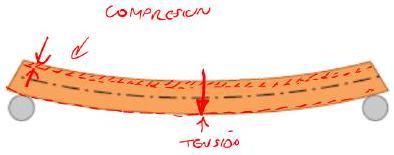
\includegraphics[max width=\textwidth, center]{2025_04_28_a9941da8947ada55c6c9g-04}

Figura 4: Barra que se pandea por su propio peso

\subsection{Esfuerzo y deformación volumétrico}
Para un esfuerzo en forma de presión casi uniforme, que actúa en todas las direcciones sobre un objeto, ocasiona un cambio de volumen, por lo que tenemos a la deformación volumétrica unitaria( $\varepsilon_{V}$ ) y el esfuerzo volumétrico $\left(\sigma_{V}\right)$. Si un objeto se sumerge en un fluido en reposo, el fluido ejerce una fuerza sobre todas las partes de la superficie del objeto; esta fuerza es perpendicular a la superficie(si fuese paralela, el fluido se deslizaría a los lados para contrarrestar la acción). Como todo objeto está sometido a una presión inicial ( $p_{0}$ ), entonces el esfuerzo volumétrico representaría el cambio de la presión ( $\sigma_{V}=\Delta p$ ). Para el caso de compresión, tenemos:\\
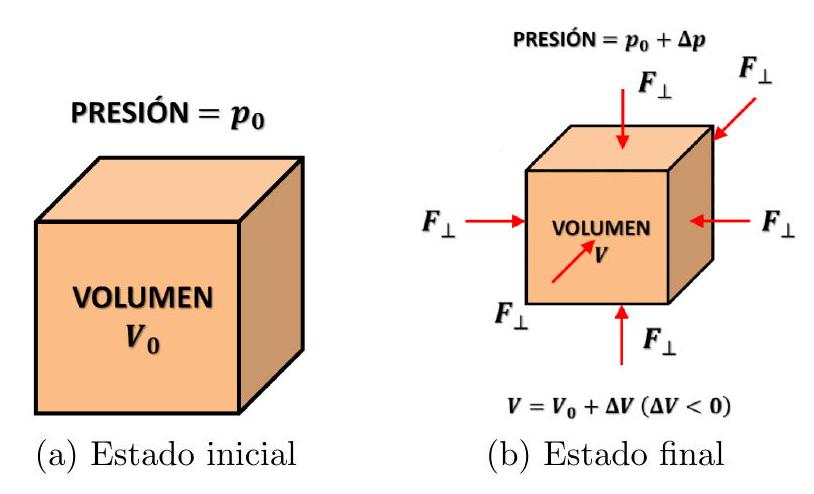
\includegraphics[max width=\textwidth, center]{2025_04_28_a9941da8947ada55c6c9g-05}

Tenemos que la deformación volumétrica unitaria es $\varepsilon_{V}=-\frac{\Delta V}{V_{0}}$. Si el cambio de presión es pequeño, entonces tenemos la ley de hooke con módulo volumétrico(B):

$$
\begin{aligned}
B & =-\frac{\sigma_{V}}{\varepsilon_{V}} \\
& =-\frac{\Delta p \cdot V_{0}}{\Delta V}
\end{aligned}
$$

\subsection{2.4. Esfuerzo y deformación por corte}
Para una situación de esfuerzo-deformación por corte, las fuerzas no actúan de forma normal a las superficies, sino que actúan de forma tangente a la superficie. Luego tenemos al esfuerzo de corte $\sigma=\frac{F_{\|}}{A}$. Entonces el objeto presenta los siguientes estados:\\
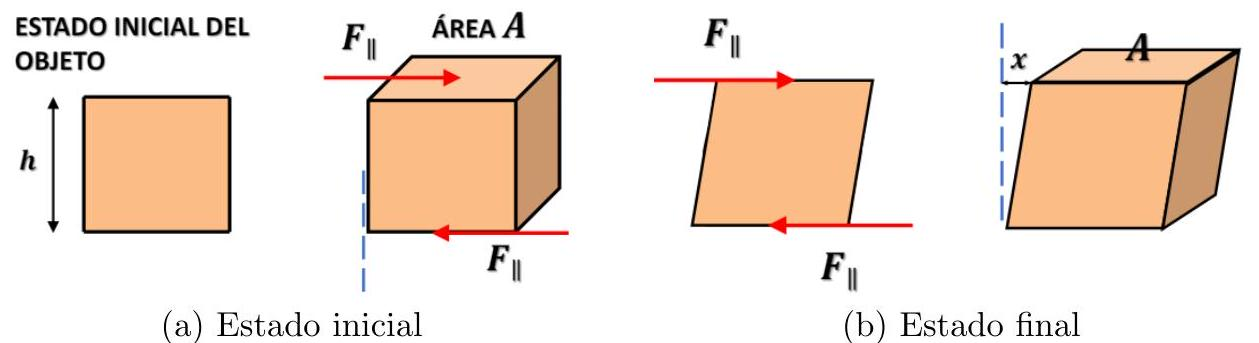
\includegraphics[max width=\textwidth, center]{2025_04_28_a9941da8947ada55c6c9g-05(1)}

Luego definimos la deformación unitaria por corte como $\varepsilon=\frac{x}{h}$. En situaciones reales\\
$x \ll h$, por lo que si las fuerzas son lo suficientemente pequeñas como para que se cumpla la ley de Hooke, entonces definimos al módulo de corte o cillazadura $(G)$ como:

$$
\begin{aligned}
G & =\frac{\sigma}{\varepsilon} \\
& =\frac{F \cdot h}{A \cdot x}
\end{aligned}
$$

Se comprueba de manera experimental y teórica que $\frac{Y}{3}<G<\frac{Y}{2}$. Tener en cuenta que estos conceptos funcionan solo para sólidos, puesto que los fluidos no tienen forma definida.

\subsection{ Deformaciones transversales}
Experimentalmente, cuando se realiza un esfuerzo de tensión, se observan deformaciones longitudinales y transversales respecto a la dirección de la fuerza. Se observa\\
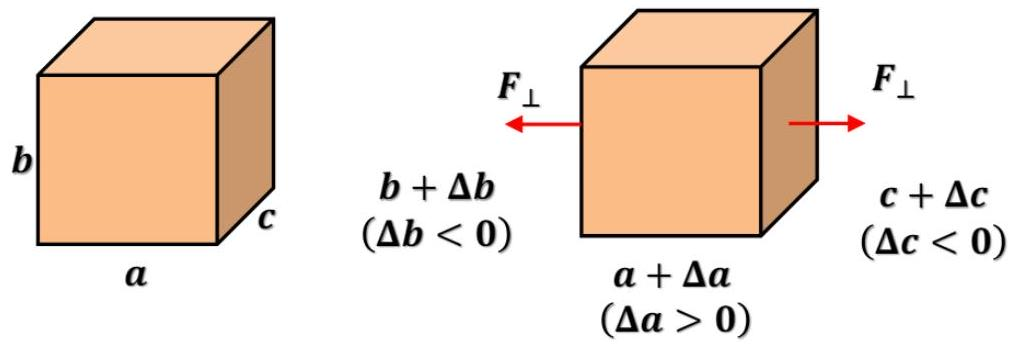
\includegraphics[max width=\textwidth, center]{2025_04_28_a9941da8947ada55c6c9g-06}

Figura 5: Objeto sometido a esfuerzo por tensión\\
que para el caso de esfuerzo por tensión, hay estiramiento longitudinal y compresiones transversales. Considerando al eje X como paralelo a la dirección de la fuerza, tenemos que el eje $Y \| b$ y el eje $Z \| c$. De esto obtenemos las deformaciones unitarias respecto a cada eje $\varepsilon_{x}=\frac{\Delta a}{a}, \varepsilon_{y}=-\frac{\Delta b}{b}$ y $\varepsilon_{z}=-\frac{\Delta c}{c}$. Considerando material isotrópico(Mismas propiedades en todas las direcciones en su interior), tenemos que $\varepsilon_{y}=\varepsilon_{z}$. Dentro de la zona elástica de un material, se tiene que la relación entre la deformación transversal unitaria y la deformación unitaria por tensión es constante(coeficiente de Poisson $\nu$ ). Luego tenemos:


\begin{equation*}
\nu=-\frac{\varepsilon_{y}}{\varepsilon_{x}} \tag{4}
\end{equation*}


Donde $\varepsilon_{y}$ es la deformación transversal y $\varepsilon_{x}$ es la deformación por tensión. Respecto a la deformación volumétrica unitaria, tomamos un elemento diferencial de dimensiones\\
$d a, d b$ y $d b$ paralelas a los ejes X, Y, Z respectivamente. Entonces tenemos:

$$
\begin{aligned}
\varepsilon & =\frac{d V}{V} \\
& =\frac{d(a b c)}{a b c} \\
& =\frac{b c d(a)+a c d(b)+a b d(c)}{a b c} \\
& =\frac{d(a)}{a}+\frac{d(b)}{b}+\frac{d(c)}{c} \\
& =\varepsilon_{x}+\varepsilon_{y}+\varepsilon_{z}
\end{aligned}
$$

Donde $\varepsilon_{x}, \varepsilon_{y} \mathrm{y} \varepsilon_{z}$ son las deformaciones unitarias totales respecto a cada eje.

\subsection{ Principio de superposición}
Si se cumple la ley de Hooke y se supone que los desplazamientos producidos por las fuerzas actuantes son muy pequeños en relación a las dimensiones del cuerpo, de tal manera que podamos considerar que mantiene la forma y dimensiones originales, entonces puede aplicarse el principio de superposición(los efectos que un sistema de fuerzas aplicadas origina en cuerpo son iguales a la suma de los efectos que originan estas fuerzas actuando por separado).\\
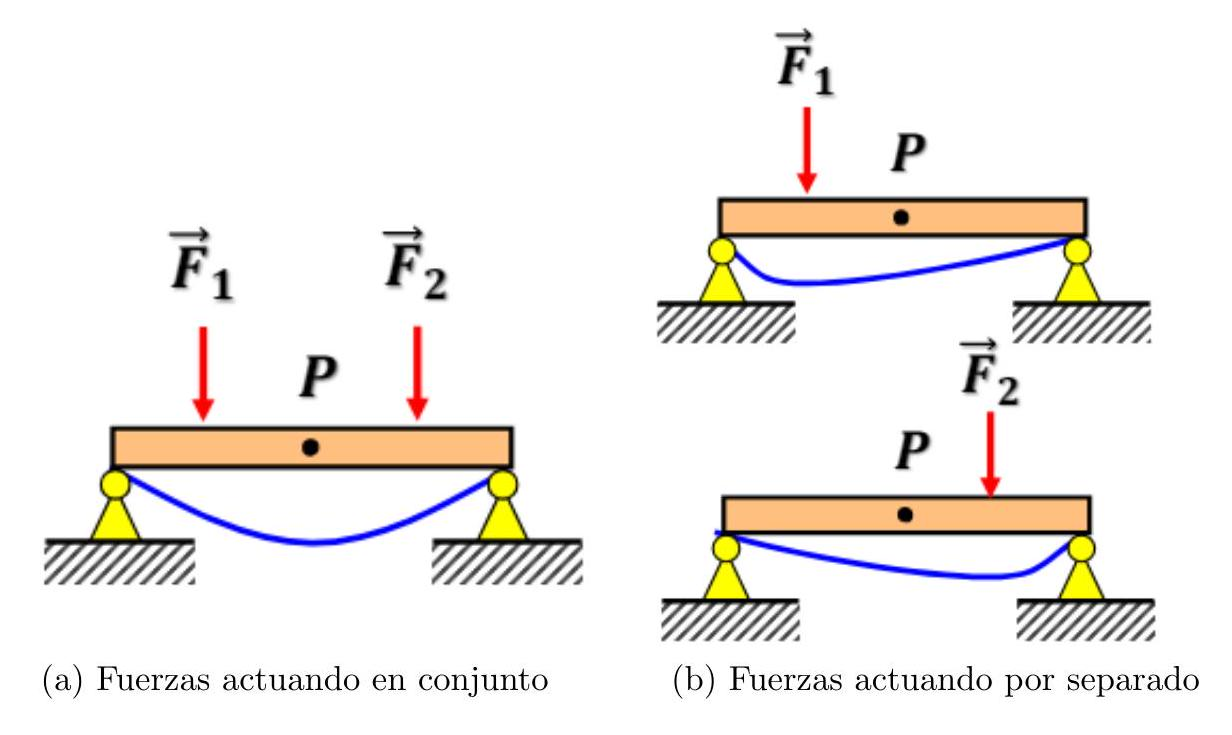
\includegraphics[max width=\textwidth, center]{2025_04_28_a9941da8947ada55c6c9g-07}

\subsection{ Elasticidad y plasticidad}
La ley de Hooke tiene un intervalo de validez. Para hallar el límite de validez, se procede a graficar el diagrama de esfuerzo-deformación. Como ejemplo, tenemos el diagrama esfuerzo-deformación típica de un metal dúctil sometido a tensión.\\
Del diagrama podemos concluir lo siguiente:\\
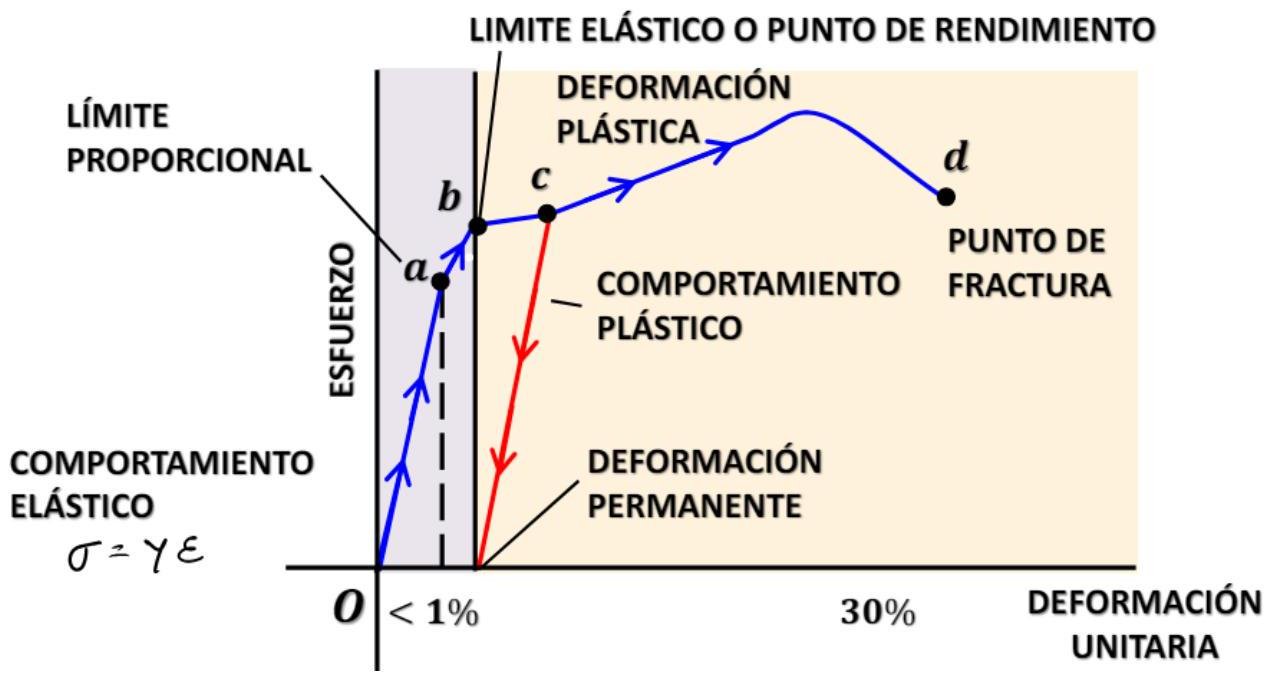
\includegraphics[max width=\textwidth, center]{2025_04_28_a9941da8947ada55c6c9g-08}

Figura 6: Diagrama esfuerzo deformación

\begin{itemize}
  \item La primera porción es una línea recta(antes de a), indicando un comportamiento acorde a la ley de Hooke.
  \item El esfuerzo en el punto a se denomina límite proporcional.
  \item Del punto a al punto b, el esfuerzo y deformación ya no son proporcionales y no se cumple la ley de Hooke, pero si la carga se retira gradualmente partiendo de cualquier punto entre O y b, se represa por la curva hasta que el material recupere su longitud original(comportamiento elástico).
  \item El esfuerzo en el punto b representa el límite elástico(o punto de rendimiento).
  \item Para un esfuerzo mayor al presente en b, se tendrá un comportamiento inelástico o plástico(el objeto no vuelve a su forma original), desplazándose por la curva hasta llegar a la parte roja y lograr deformación permanente.
  \item Para un esfuerzo más allá del presente en c, tenemos que en d se llega a la fractura.
  \item El comportamiento entre b y d se denomina flujo plástico o deformación plástica.
\end{itemize}

\subsection{Histéresis elástica}
Para un objeto que se estira y luego se deja relajar, puede llegar a ocurrir algo muy excepcional. Tomando de ejemplo a una curva esfuerzo-deformación de caucho vulcanizado estirado a más de siete veces su longitud original, tenemos:\\
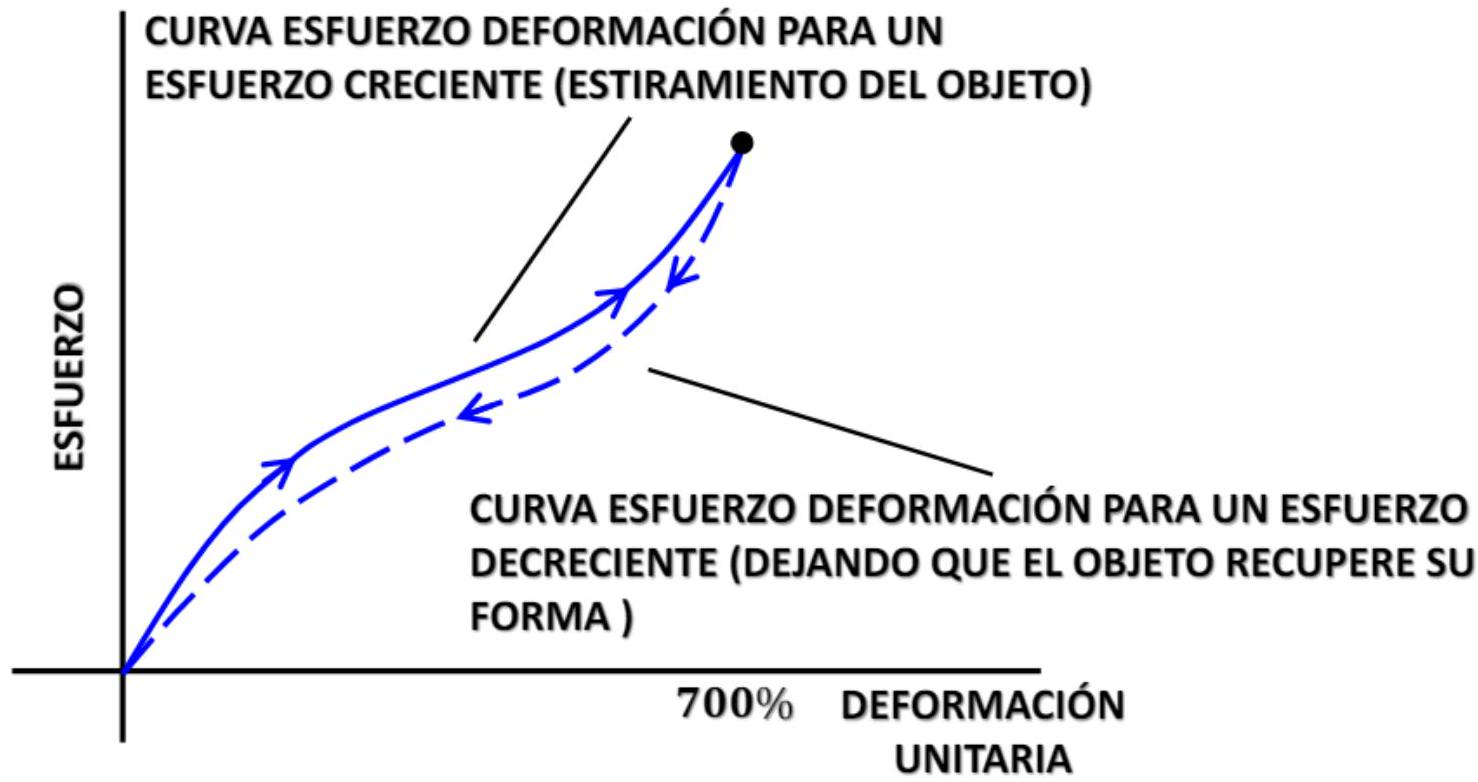
\includegraphics[max width=\textwidth, center]{2025_04_28_a9941da8947ada55c6c9g-09}

Figura 7: Diagrama esfuerzo-deformación para el caucho vulcanizado

Se observa que el esfuerzo no es proporcional a la deformación, pero el comportamiento es elástico. Se observa también que el material sigue curvas diferentes respecto a aumento y disminución del esfuerzo. Esto se denomina histéresis elástica.

\subsection{ Aplicaciones al experimento}
Para lograr el objetivo principal del experimento, se hará uso de la teoría anteriormente presentada, diferenciando el esfuerzo técnico como $\sigma_{0}=\frac{F}{S_{0}}(F$ es la fuerza perpendicular a la superficie y $S_{0}$ es el área inicial de la sección transversal del objeto) y al esfuerzo real como $\sigma=\frac{F}{S}$ ( $S$ es el área final de la sección transversal del objeto). Para el experimento, se utilizarán masas, de modo que el esfuerzo y deformación unitaria se acomoden a la ley de Hooke y halla un comportamiento elástico.

